%% 
%% Latex Practice
%% Use https://tikzcd.yichuanshen.de/ for diagrams
%leqno,fleqn,
\documentclass[10pt,letterpaper]{article}


\usepackage[comma,authoryear]{natbib}
\usepackage{float}
\usepackage{graphicx}
\usepackage{setspace}
% \usepackage{kpfonts}
\usepackage{textcomp}
% \usepackage{fullpage}
\usepackage{url}
\usepackage[usenames,dvipsnames,svgnames,table]{xcolor}
%\usepackage{mdframed}  % not availble on ubuntu

% -- font styles
\usepackage{tgtermes}
% \usepackage[lf]{venturis}
% \usepackage{times}
% \usepackage[sc]{mathpazo} % Palatino (very readable)
% \usepackage[adobe-utopia]{mathdesign}
% \usepackage{gfsdidot}
% \usepackage[scaled]{beraserif}
% \usepackage[bitstream-charter]{mathdesign}
% \usepackage{mathptmx}
\usepackage{enumitem}
% some more math stuff/ diagrams
\usepackage{amssymb}
\usepackage{tikz-cd}
% special math formatting
\usepackage{amsmath}

\floatstyle{ruled}

% -- structural elements
\newfloat{program}{thp}{lop}
\floatname{program}{Program}

%\newfloat{figure}{thp}{lop}
%\floatname{figure}{Figure}

% -- syntax highlighting
\usepackage{listings}
  \usepackage[scaled]{beramono}
  \usepackage[T1]{fontenc}
\usepackage{color}

\usepackage{caption}
% -- configure captions for figures
\DeclareCaptionFormat{listing}{\par\hrule #1#2#3}
\captionsetup[figure]{%
  format=listing, 
  singlelinecheck=false, 
  margin=00pt, 
  font={it,footnotesize,centering}
}

\parskip 12pt

% page margins
\setlength{\textheight}{22cm}
\setlength{\oddsidemargin}{0.25in}
\setlength{\textwidth}{6in}

% I don't know what this does
\def\printcitestart{\unskip $^\bgroup}
\def\printbetweencitations{,}
\def\printcitefinish{\egroup$}
\def\printcitenote#1{\hbox{\sevenrm\space (#1)}}


% TODO: mdframed doesn't work well with ubuntu
% \newenvironment{aside}
%   {\begin{mdframed}[style=0,%
%       leftline=false,rightline=false,leftmargin=2em,rightmargin=2em,%
%           innerleftmargin=0pt,innerrightmargin=0pt,linewidth=0.75pt,%
%       skipabove=25pt,skipbelow=25pt]\small}
%   {\end{mdframed}}


%% Bibliography configuration
%% ------------------------------
\bibliographystyle{apalike}
% don't show reference label in the bibliography (APA specific)
\makeatletter
\def\@biblabel#1{}
\makeatother


\lstset{
  %framesep=5pt,
  upquote=true,
  breaklines=false,
  %postbreak=\raisebox{0ex}[0ex][0ex]{\ensuremath{\hookrightarrow}},
  breakatwhitespace=true,
  %numbers=left,
  language=Java,
  basicstyle=\footnotesize\ttfamily,
  numberstyle=\footnotesize\ttfamily,
  %numbersep=10pt,
  tabsize=2,
  extendedchars=true,
  showtabs=false,
  showspaces=false,
  showstringspaces=false,
  xleftmargin=20pt,
  aboveskip=10pt,
  % colors
  stringstyle=\color{Maroon},
  commentstyle=\color{Gray},
  rulecolor=\color{Gray},
  keywordstyle=\color{Blue},
  %backgroundcolor=\color{LightGray!.50}
}
\lstloadlanguages{
  Java
}


% Hyphenation rules ------------
%% \hyphenation{Fire-Detection-System}
%% \hyphenation{Emergency-Communication-System}


\title{Algorithm Design Manual Notes}
\author{Zachary William Grimm\\
  \small{Notes  for ADM by Skiena}\\
  \small{zwgrimm@gmail.com}
}
\date{\today{}}

\begin{document}

\setstretch{1.00}
\maketitle

% -- Table of Contents --
\tableofcontents{}

\newpage{}
 
% -- set document spacing --
% \setstretch{1.09}  % single line
% \setstretch{1.30}  % single wide-spaced\subsubsection*{\textbf{1-12.} \emph{Prove that $\sum_{i=1}^{n}i^{3}=\frac{n^{2}(n+1)^{2}}{4} \;for\; n \geq 0$, by induction}}
% \setstretch{1.50}  % one and a half spacing

% -- Import content here
\section{Introduction To Algorithm Design}
the algorithmic \emph{problem} known as \emph{sorting} is defined as follows: \\
\emph{Problem:} Sorting \\
\emph{Input:} A sequence of n keys $a_{1},...,a_{n}$. \\
\emph{Output:} The permutation (reordering) of the input sequence such that $a_{1}^{'} \leq a_{2}^{'} \leq ... \leq a_{n-1}^{'} \leq a_{n}^{'}$\\


\noindent\rule{\textwidth}{0.4pt}

\begin{figure}[H]
  \centering
     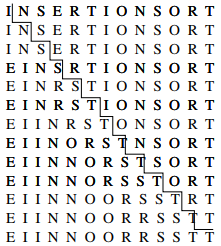
\includegraphics[scale=0.6]{./insertion_sort.png}
  \label{fig:demo-diagram}
  \caption{Animation of insertion sort in action (time flows down)}
\end{figure}


\begin{verbatim}
insertion_sort(item s[], int n)
{
    int i,j; /* counters */

    for (i=1; i<n; i++) {
        j=i;
        while ((j>0) && (s[j] < s[j-1])) {
            swap(&s[j], &s[j-1]);
            j = j-1;
        }
    }
}
\end{verbatim}

\noindent\rule{\textwidth}{0.4pt}


\begin{figure}[H]
  \centering
     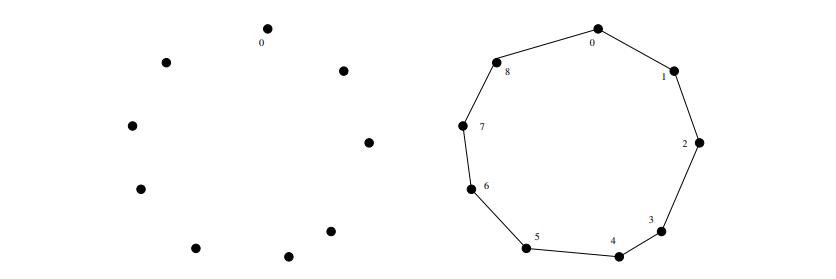
\includegraphics[scale=0.6]{./nearest_neighbor.png}
  \label{fig:demo-diagram2}
  \caption{A good instance for the nearest neighbor heuristic}
\end{figure}




\subsection{Robot Tour Optimization}
aaa
\subsection{Selecting the Right Jobs}
bbb

\subsubsection{test, delete this}
\subsection{Reasoning about Correctness}

\subsubsection{Expressing Algorithms}
\subsection{Modeling The Problem}

\subsubsection{Combinatorial Objects}

\subsubsection{Recursive Objects}
\subsection{About the War Stories}


\subsection{War Story: Psychic Modeling}

\section{Algorithm Analysis}
Our two most important tools are 
\begin{enumerate}
	\item
	  \emph{The RAM model of
			computation}
	\item
	  \emph{The asymptotic analysis of worst-case complexity}
\end{enumerate}

\subsection{The RAM Model of Computation}

\subsubsection{Best, Worst, and Average-Case Complexity}

\subsection{The Big Oh Notation}
\subsection{Growth Rates and Dominance Relations}

\begin{figure}[H]
  \centering
     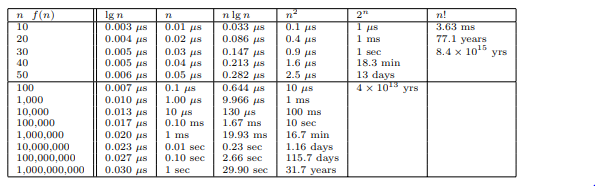
\includegraphics[scale=1.0]{./2_4.png}
  \label{fig:demo-diagram2-4}
  \caption{ Growth rates of common functions measured in nanoseconds}
\end{figure}


\subsubsection{Dominance Relations}

\noindent\fbox{\parbox{\textwidth}{%
\emph{Take-Home Lesson: }Although esoteric functions arise in advanced algorithm
analysis, a small variety of time complexities suffice and account for most
algorithms that are widely used in practice.
}%
}



\subsection{Working with the Big Oh}

\subsubsection{Adding Functions}

$$O(f(n)) + O(g(n)) \longrightarrow O(max(f(n),g(n))$$

$$\Omega(f(n)) + \Omega(g(n)) \longrightarrow \Omega(max(f(n),g(n))$$


$$\Theta(f(n)) + \Theta(g(n)) \longrightarrow \Theta(max(f(n),g(n))$$

\subsubsection{Multiplying Functions}

$$O(c*f(n))) \longrightarrow O(f(n))$$

$$\Omega(c*f(n))) \longrightarrow \Omega(f(n))$$


$$\Theta(c*f(n))) \longrightarrow \Theta(f(n))$$

\noindent\rule{\textwidth}{0.4pt}

$$O(f(n)) * O(g(n)) \longrightarrow O(f(n) * g(n))$$

$$\Omega(f(n)) * \Omega(g(n)) \longrightarrow \Omega(f(n) * g(n))$$

$$\Theta(f(n)) * \Theta(g(n)) \longrightarrow \Theta(f(n) * g(n))$$

\noindent\rule{\textwidth}{0.4pt}

\textbf{Stop and Think: Hip to the SquaresTransitive Experience} \\

\emph{Show that Big Oh relationships are transitive. That is, if $f(n) = O(g(n))$ and $g(n) = O(h(n))$, then $f(n) = O(h(n))$}
\subsection{Reasoning About Efficiency}

\subsubsection{Selection Sort}

\subsubsection{Insertion Sort}

\subsubsection{String Pattern Matching}

\subsubsection{Matrix Multiplication}
\subsection{Logarithms and Their Applications}
$$b^{x} = y \leftrightarrow x = log_{b}y$$
$$b^{log_{b}y} = y$$

\subsubsection{Logarithms and Binary Search}

\begin{figure}[H]
  \centering
     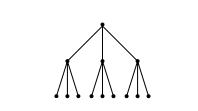
\includegraphics[scale=0.9]{./2_7.png}
  \label{fig:demo-diagram2-4}
  \caption{ A height \emph{h} tree with \emph{d} children per node as \emph{$d^{h}$} leaves. Here $h=2$ and $d=3$}
\end{figure}


\subsubsection{Logarithms Trees}

\subsubsection{Logarithms and Bits}

\subsubsection{Logarithms and Multiplication}

\begin{align*}
	&log_{a}(xy) = log_{a}(x) + log_a(y) \\
	&log_{a} n^{b} = b \cdot log_{a} n \\
	&a^{b} = e^{(ln(a^{b}))} = e^{(b(ln(a)))}
\end{align*}

\subsubsection{Fast Exponentiation}

\subsubsection{Logarithms and Summations}

\emph{Harmonic Numbers}: 
$$H(n) = \sum_{i=1}^{n} \frac{1}{i} \sim ln(n)$$

\subsubsection{Logarithms and Criminal Justice}


\begin{figure}[H]
  \centering
     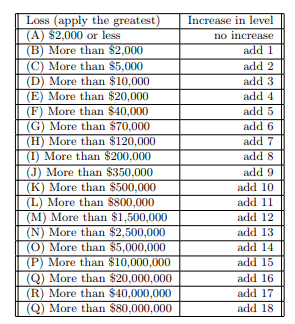
\includegraphics[scale=0.9]{./2_8.png}
  \label{fig:demo-diagram2-8}
  \caption{The Federal Sentencing Guidelines for fraud}
\end{figure}

\noindent\fbox{\parbox{\textwidth}{%
\emph{Take-Home Lesson: } Logarithms arise whenever things are repeatedly halved or doubled
}%
}

\subsection{Properties of Logarithms}

$$log_{a}b = \frac{log_{c}b}{log_{c}a}$$

\textbf{Stop and Think: Importnce of an Even Split} \\

\emph{How many queries does binary search take on the million-name Manhattan phone boo if each split was 1/3 to 2/3 instead of 1/2 to 1/2?}
\subsection{War Story: Mystery of the Pyramids}
\subsection{Advanced Aanalysis (*)}

\subsection{Esoteric Functions}

\subsection{Limits and Dominance Relations}

\noindent\fbox{\parbox{\textwidth}{%
\emph{Take-Home Lesson: } By interleaving the functions here with those of Section 2.3.1 we see where everything fits into the dominnce pecking order:
$$n! \gg c^{n} \gg n^{3} \gg n^{2} \gg n^{1 + \epsilon} \gg n\cdot log(n) \gg n \gg \sqrt{n}$$
$$ \gg log^{2}n \gg log(n) \gg \frac{log(n)}{log(log(n))} \gg log(log(n)) \gg \alpha (n) \gg 1$$
}%
}

\section{Data Structures}
% 3 Fundamental abstract data types

\begin{itemize}
	\item \emph{Containers}
	\item \emph{Dictionaries}
	\item \emph{Lists}
\end{itemize}
\subsection{Contigous vs. Linked Data Structures}

\begin{itemize}
	\item 
	  \emph{Continuously allocated structures (arrays)}
	\item 
	  \emph{Linked data structures (pointers, lists, trees...)}
\end{itemize}

\subsubsection{Arrays}
$$M=\sum_{i=1}^{lg(n)} i*\frac{n}{2^{i}} = n*\sum_{i=1}^{lg(n)}\frac{i}{2^{i}} \leq n*\sum_{i=1}^{\infty}\frac{i}{2^{i}} = 2n$$

\subsubsection{Pointers and Linked Structures}

figure here*** (Linked Lst example showing data and pointer fields)

\begin{verbatim}
  typedef struct list {
    item_type item;          /*data item*/
    struct list *next;       /*point to successor*/
  } list;
\end{verbatim}

\textbf{ \emph{Searching a List} }\\

\begin{verbatim}
  list *search_list(list *1, item_type x)
  {
    if(1 == NULL) return(NULL);

    if(1->item == x)
      return(1);
    else
      return(search_list(1->next, x) );
  }
\end{verbatim}

\textbf{ \emph{Insertion into a List} }\\

\begin{verbatim}
  void insert_list(list **1, item_type x) 
  {
      list *p                  /* temporary pointer*/

      p = malloc(sizeof(list));
      p->item = x;
      p->next = *1;
      *1 = p;
  }
\end{verbatim}

\textbf{ \emph{Deletion From a List} }\\

\begin{verbatim}
  list *predecessor_list(list *1, item_type x)
  {
      if((1 == NULL) || (1->next == NULL)) {
          printf("Error: predecessor sought on null list.\n");
          return(NULL);
      }

      if((1->next)->item == x)
          return(1);
      else
          return(predecessor_list(1->next, x));
  }

  delete_list(list **1, item_type x)
  {
      list *p;                      /*item pointer*/
      list *pred                    /*predecessor pointer*/
      list *search_list(), *predecessor_list();

      p = search_list(*1,x);
      if(p != NULL) {
          pred = predecessor_list(*1, x);
          if(pred == NULL)          /*splice out list*/
              *1 = p->next;
          else
              pred->next = p->next;
          free(p);                  /*free memory used by node*/
      }
  }
\end{verbatim}

\subsubsection{Comparison}

\noindent\fbox{\parbox{\textwidth}{%
\emph{Take-Home Lesson: }Dynamic memory allocation provides us with flexibility on how and where we use our limited storage resources.
}%
}







% -- Bibliography (APA)
% \bibliography{references}

\end{document}